\subsection{perceptual coding}	
	\begin{frame}{source coding}{perceptual coding: introduction}
        \begin{itemize}
            \item   \textbf{goal}: 
                \begin{itemize}
                    \item   encode signal in a way that the decoded signal is \textbf{perceptually} as close to the original signal as possible
                \end{itemize}
            \pause
            \bigskip
            \item   \textbf{common codecs}:
                \begin{itemize}
                    \item   MPEG-1/2 Layer 2
                    \item   MPEG-1/2 Layer 3
                    \item   %\color<5->{gtgold}{
                    MPEG-2/4 AAC
                    \item   AC-3/4
                    \item   Ogg Vorbis
                    \item   (DTS  Cine/Home)
                    \item   (ATRAC)
                \end{itemize}
        \end{itemize}
	\end{frame}
	\begin{frame}{source coding}{perceptual coding: overview}
        \vspace{-5mm}
        \begin{figure}
			\begin{center}
	            \begin{picture}(90,70)
	
	                %boxes \colorbox{gray!20}
	                \put(0,40){\framebox (20,10){\scriptsize\color<2>{gtgold}\shortstack[c]{Psychoacoustic\\ Model}}}
	                \put(0,0){\framebox (20,10){\scriptsize\shortstack[c]{Bit Allocation}}}

	                \put(30,40){\framebox (20,10){\scriptsize\shortstack[c]{Frequency\\ Transformation}}}
	                \put(30,20){\framebox (20,10){\scriptsize\shortstack[c]{Additional\\ Processing}}}
	                \put(30,0){\framebox (20,10){\scriptsize\shortstack[c]{Quantization\\ Entropy Coding}}}
	
	                \put(60,0){\framebox (20,50){\scriptsize\shortstack[c]{Bitstream\\ Formatting}}}

	                %lines horizontal
	                \put(10,25){\vector(1,0){20}}
	                \put(20,5){\vector(1,0){10}}
	                \put(10,60){\line(1,0){30}}

	                \put(50,45){\vector(1,0){10}}
	                \put(50,25){\vector(1,0){10}}
	                \put(50, 5){\vector(1,0){10}}

	                \put(80,25){\vector(1,0){5}}
	
	                %lines vertical
	                \put(10,60){\vector(0,-1){10}}
	                \put(10,40){\vector(0,-1){30}}

	                \put(40,65){\vector(0,-1){15}}
	                \put(40,40){\vector(0,-1){10}}
	                \put(40,20){\vector(0,-1){10}}
	                
	                %circles
	                \put(10,25){\circle*{1}}

	                \put(40,60){\circle*{1}}
	
	                %text
	                \put(42,65){\footnotesize{\shortstack[c]{input}}}
	                \put(84,27){\footnotesize{\shortstack[c]{bitstream}}}
	            \end{picture}
			\end{center}
	    \end{figure}
	\end{frame}
	
	\begin{frame}{source coding}{psycho-acoustic model: overview}
        \begin{itemize}
            \item   \textbf{objective}:\\ identify components perceptible and imperceptible by humans
            \pause
            \smallskip
            \item   \textbf{approach}:\\ build model of human sound perception (\textit{analysis only!})
            \pause
            \smallskip
            \item   \textbf{processing steps}:
                \begin{enumerate}
                    \item	transform to \textbf{frequency domain}
                    \pause
                    \item	map to \textbf{perceptual frequency scale}
                    \pause
                    \item   group into bands
                    \pause
                    \item	compute (perceptual) \textbf{masking threshold}
                    \pause
                    \item	compute \textbf{Signal-to-Mask Ratio} (SMR)
                    \pause
                    \item   compute additional analysis results
                \end{enumerate}
            \pause
            \smallskip
            \item   \textbf{recommendation only}! no specific standardization
        \end{itemize}
	\end{frame}
	
	\begin{frame}{source coding}{psycho-acoustic model 1--3: frequency transform}
		\begin{itemize}
            \item   frequency transformation (AAC: FFT)
            \item   frequency warping and grouping of power in bands (AAC: Bark scale with \nicefrac{1}{3} Bark resolution)
            \begin{figure}
				\centering
					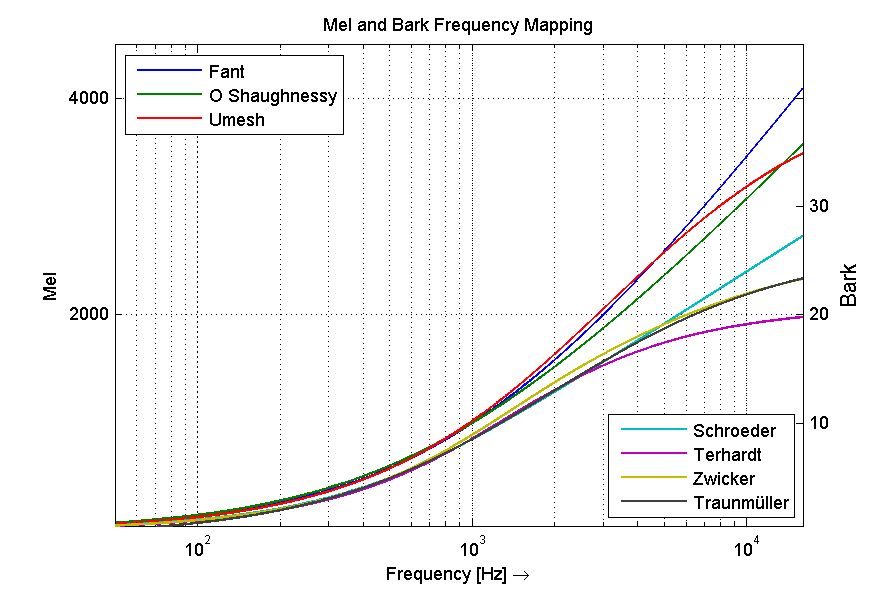
\includegraphics[scale=0.6]{Graph/mel}
			\end{figure}
        \end{itemize}
	\end{frame}
	
	\begin{frame}{source coding}{psycho-acoustic model 4: masking threshold 1/2}
        \begin{itemize}
            \item   humans are not able to perceive every possible detail in an audio signal
                \begin{enumerate}
                    \item<1->   frequency resolution (see above)
                    \item<1->   sensitivity for specific frequency regions
                        \only<1>{
                        \begin{figure}
                            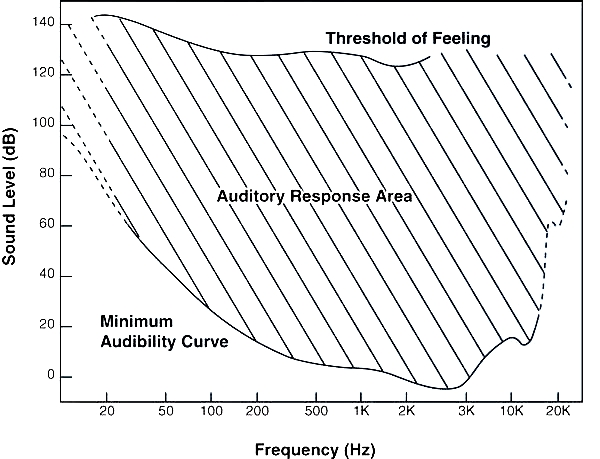
\includegraphics[scale=.25]{graph/hearingarea}
                        \end{figure}}
                    \item<2->   components masked by other components
                         \only<2>{
                        \begin{figure}
                            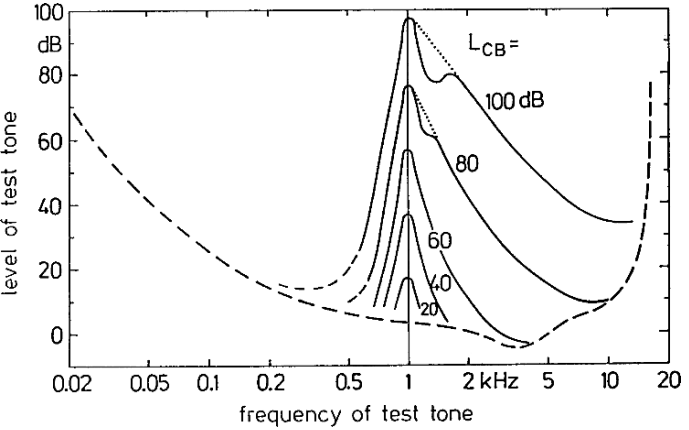
\includegraphics[scale=.25]{graph/maskingtonebynarrownoise2}
                            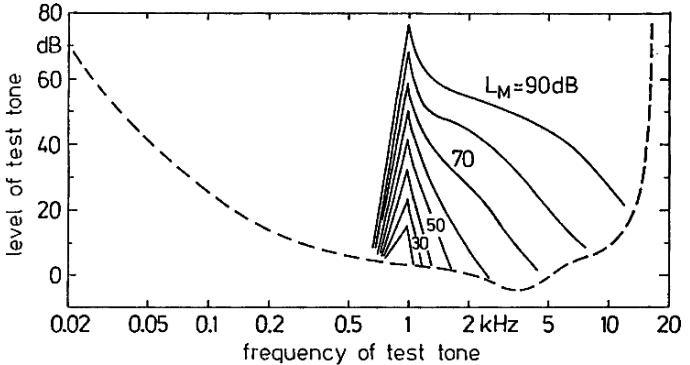
\includegraphics[scale=.25]{graph/maskingtonebytone}
                            
                            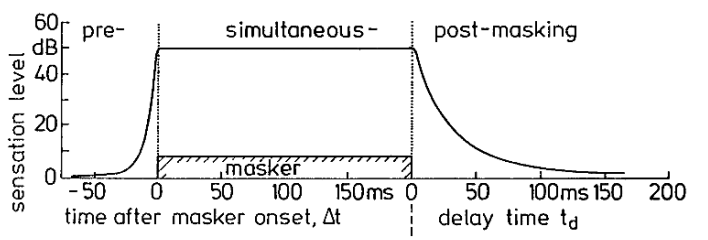
\includegraphics[scale=.25]{graph/maskingtemporal}
                        \end{figure}}
                    \item<3->   masking threshold depends on
                            \begin{itemize}
                                \item   \textit{frequency} of masker
                                \item   \textit{noisiness} of masker
                                \item   \textit{level} of masker
                                \item   \textit{duration} of masker
                            \end{itemize}
               \end{enumerate}
        \end{itemize}
        \vspace{70mm}
	\end{frame}
	
	\begin{frame}{source coding}{psycho-acoustic model 4: masking threshold 2/2}
        AAC computation of masking threshold (recommendation)
        \begin{itemize}
            \item       take hearing threshold as minimum masking threshold
            \item<2->   convolve band spectrum with spreading function
                        \uncover<2->
                        {
                        \begin{figure}
                            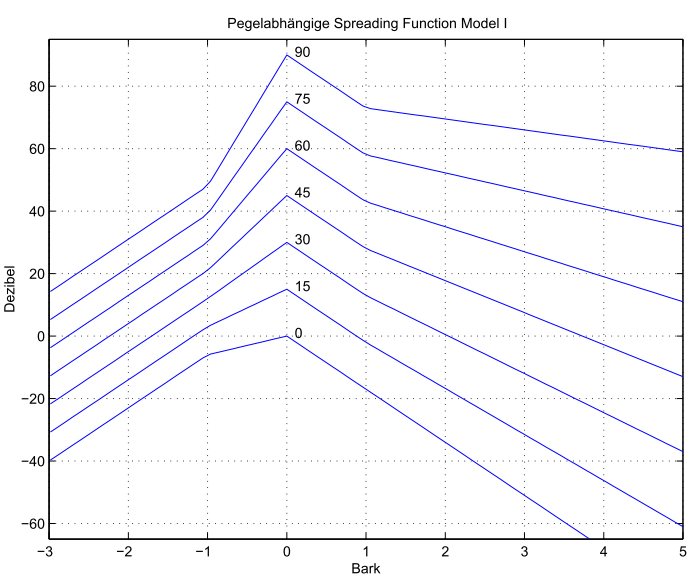
\includegraphics[scale=.25]{graph/spreadingfunction_layer2}
                            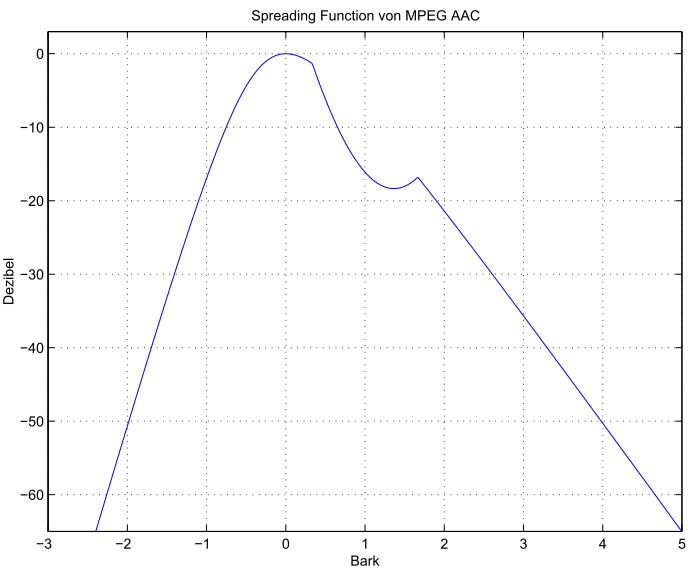
\includegraphics[scale=.25]{graph/spreadingfunction_aac}
                        \end{figure}}
            \item<3->   compute tonality (with phase deviation) and apply to masking threshold (from original spectrum)
        \end{itemize}
        
	\end{frame}
	
	\begin{frame}{source coding}{psycho-acoustic model: visualization}
			\begin{figure}
				\centering
					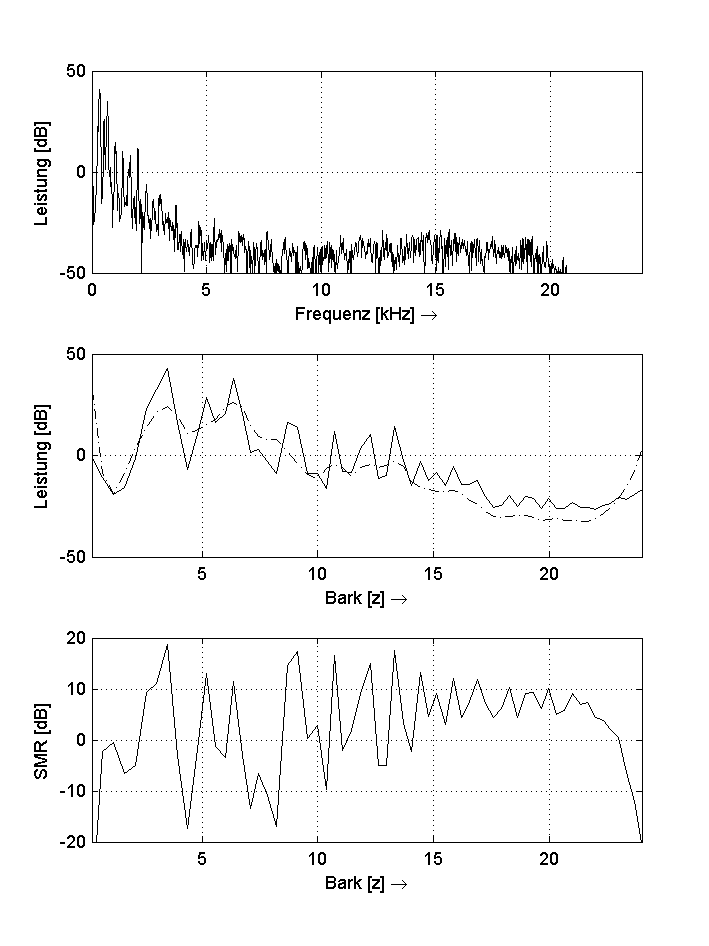
\includegraphics[scale=0.4]{Graph/Lerch16-8}
					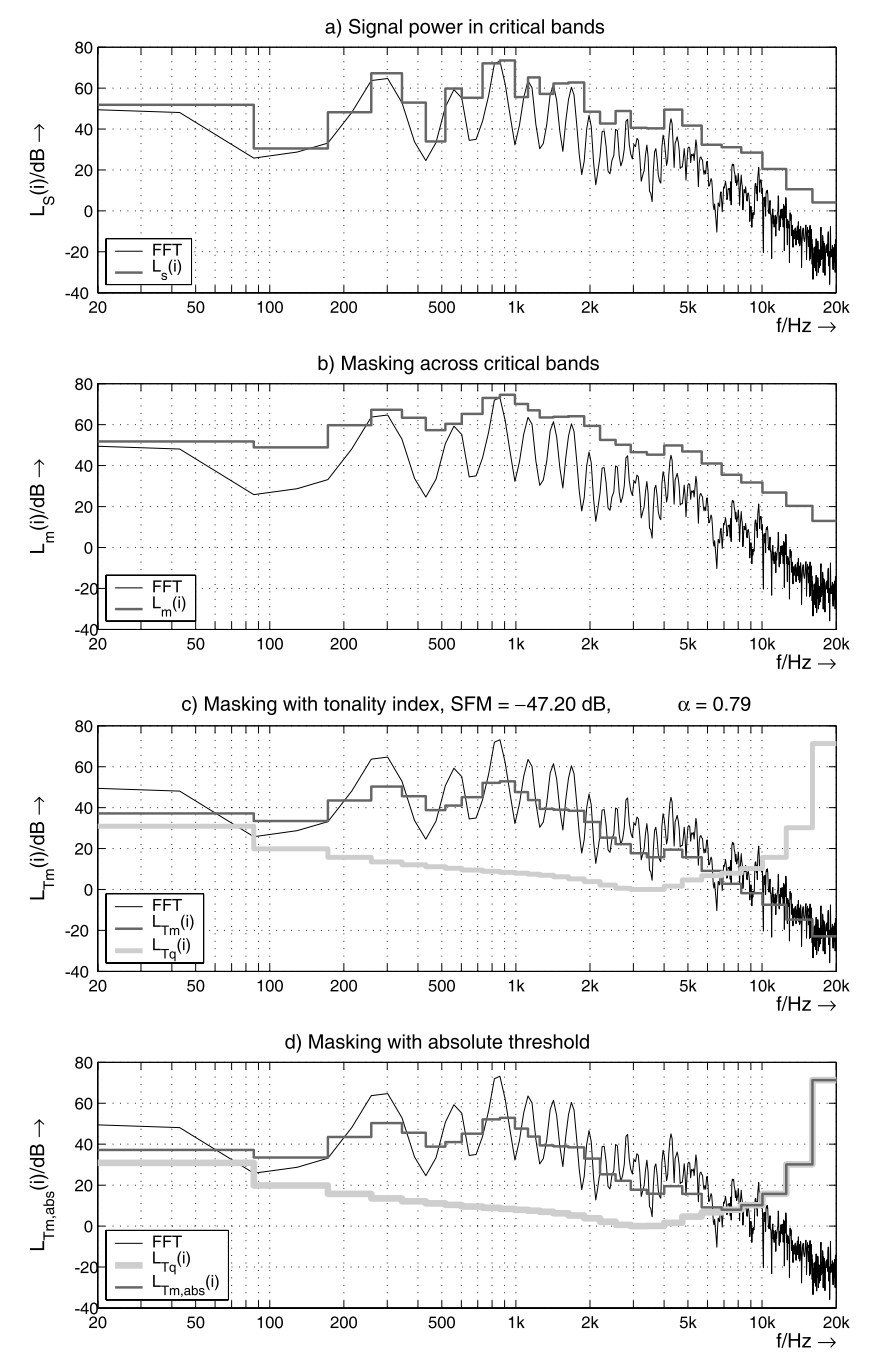
\includegraphics[scale=0.2]{Graph/psychomodeloutput}
			\end{figure}
	\end{frame}
	
	\begin{frame}{source coding}{psycho-acoustic model 6: additionally extracted information}
        \begin{itemize}
            \item   control of
                \begin{itemize}
                    \item \textbf{window length switching}
                    \item   \textbf{bit reservoir} 
                    \item   \textbf{joint stereo parameters}
                \end{itemize}
        \end{itemize}
	\end{frame}
	\begin{frame}{source coding}{perceptual coding: overview}
        \vspace{-5mm}
        \begin{figure}
			\begin{center}
	            \begin{picture}(90,70)
	
	                %boxes \colorbox{gray!20}
	                \put(0,40){\framebox (20,10){\scriptsize\shortstack[c]{Psychoacoustic\\ Model}}}
	                \put(0,0){\framebox (20,10){\scriptsize\color<1>{gtgold}\shortstack[c]{Bit Allocation}}}

	                \put(30,40){\framebox (20,10){\scriptsize\shortstack[c]{Frequency\\ Transformation}}}
	                \put(30,20){\framebox (20,10){\scriptsize\shortstack[c]{Additional\\ Processing}}}
	                \put(30,0){\framebox (20,10){\scriptsize\color<1>{gtgold}\shortstack[c]{Quantization\\ Entropy Coding}}}
	
	                \put(60,0){\framebox (20,50){\scriptsize\shortstack[c]{Bitstream\\ Formatting}}}

	                %lines horizontal
	                \put(10,25){\vector(1,0){20}}
	                \put(20,5){\vector(1,0){10}}
	                \put(10,60){\line(1,0){30}}

	                \put(50,45){\vector(1,0){10}}
	                \put(50,25){\vector(1,0){10}}
	                \put(50, 5){\vector(1,0){10}}

	                \put(80,25){\vector(1,0){5}}
	
	                %lines vertical
	                \put(10,60){\vector(0,-1){10}}
	                \put(10,40){\vector(0,-1){30}}

	                \put(40,65){\vector(0,-1){15}}
	                \put(40,40){\vector(0,-1){10}}
	                \put(40,20){\vector(0,-1){10}}
	                
	                %circles
	                \put(10,25){\circle*{1}}

	                \put(40,60){\circle*{1}}
	
	                %text
	                \put(42,65){\footnotesize{\shortstack[c]{input}}}
	                \put(84,27){\footnotesize{\shortstack[c]{bitstream}}}
	            \end{picture}
			\end{center}
	    \end{figure}
	\end{frame}
	
	\begin{frame}{source coding}{perceptual coding: bit allocation}
		\begin{itemize}
			\item	\textbf{bit allocation}
				\begin{itemize}
                    \item   how many bits are \textbf{required} (SMR)?
                        \begin{itemize}
                            \item   exact number is unknown (Entropy coding!)
                        \end{itemize}
					\item	how many bits are \textbf{available} per block?
					\item	are there bits available in the \textbf{bit reservoir} ($\approx 6000 bits$, bit rate dependent)
                        \begin{itemize}
                            \item   actual rate must never exceed channel capacity
                            \item   some frames might need more bits to properly encode
                            \item   allow deviation from constant bitrate 
                            \item   has to be allocated from previous frames 
                            \item   causes additional decoder delay
                        \end{itemize}
					\item	intelligently distribute available bits over bands 
				\end{itemize}
		\end{itemize}
        \begin{figure}
            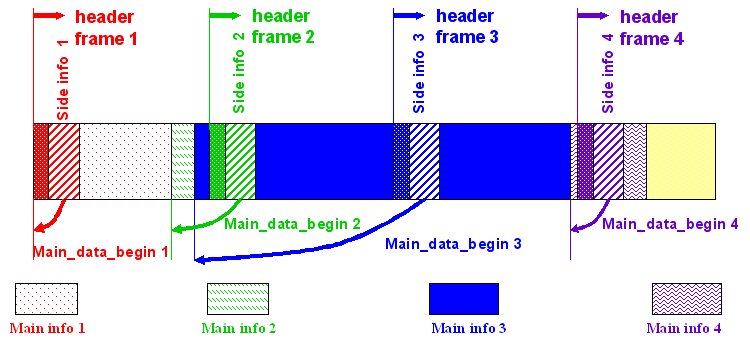
\includegraphics[scale=.2]{graph/bit_reservoir}
        \end{figure}
	\end{frame}
	
	\begin{frame}{source coding}{perceptual coding: quantization \& entropy coding}
		\begin{itemize}
			\item	\textbf{quantization}
				\begin{itemize}
					\item	re-quantize the spectrum per band
					\item	each band has different \textit{scaling factor} and \textit{word length}
                    \item   non-uniform quantization
				\end{itemize}
			\pause
			\bigskip
            \item	\textbf{entropy coding}
				\begin{itemize}
					\item	apply lossless coding (multiple dictionaries)
					\item	submit the gained bits to bit allocation (re-iterate?)
				\end{itemize}
		\end{itemize}
	\end{frame}
	
	\begin{frame}{source coding}{perceptual coding artifacts: transient smearing and pre-echo}
			\begin{figure}
				\centering
					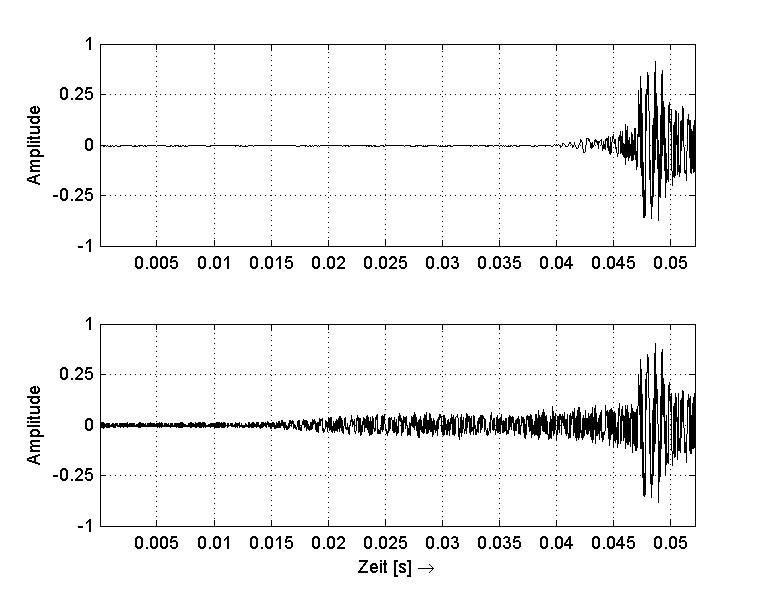
\includegraphics[scale=0.5]{Graph/Lerch16-9}
			\end{figure}
	\end{frame}
	
	\begin{frame}{source coding}{perceptual coding tweaks: block switching}
			\begin{figure}
				\centering
					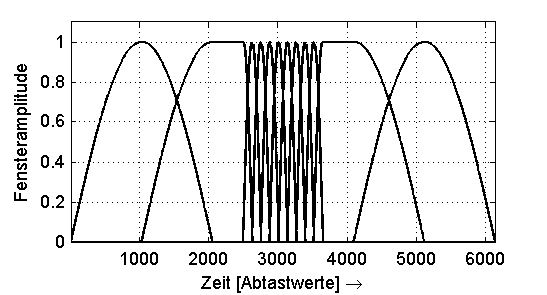
\includegraphics[scale=0.9]{Graph/Lerch16-4}
			\end{figure}
            \begin{itemize}
                \item   AAC: transients are encoded by 8 short frames (256) instead of 1 long frame (2048)
                \item   introduces encoding delay because of different start window shape
            \end{itemize}
	\end{frame}
    
	\begin{frame}{source coding}{perceptual coding: overview}
        \vspace{-5mm}
        \begin{figure}
			\begin{center}
	            \begin{picture}(90,70)
	
	                %boxes \colorbox{gray!20}
	                \put(0,40){\framebox (20,10){\scriptsize\shortstack[c]{Psychoacoustic\\ Model}}}
	                \put(0,0){\framebox (20,10){\scriptsize\shortstack[c]{Bit Allocation}}}

	                \put(30,40){\framebox (20,10){\scriptsize\shortstack[c]{Frequency\\ Transformation}}}
	                \put(30,20){\framebox (20,10){\scriptsize\color<1>{gtgold}\shortstack[c]{Additional\\ Processing}}}
	                \put(30,0){\framebox (20,10){\scriptsize\shortstack[c]{Quantization\\ Entropy Coding}}}
	
	                \put(60,0){\framebox (20,50){\scriptsize\shortstack[c]{Bitstream\\ Formatting}}}

	                %lines horizontal
	                \put(10,25){\vector(1,0){20}}
	                \put(20,5){\vector(1,0){10}}
	                \put(10,60){\line(1,0){30}}

	                \put(50,45){\vector(1,0){10}}
	                \put(50,25){\vector(1,0){10}}
	                \put(50, 5){\vector(1,0){10}}

	                \put(80,25){\vector(1,0){5}}
	
	                %lines vertical
	                \put(10,60){\vector(0,-1){10}}
	                \put(10,40){\vector(0,-1){30}}

	                \put(40,65){\vector(0,-1){15}}
	                \put(40,40){\vector(0,-1){10}}
	                \put(40,20){\vector(0,-1){10}}
	                
	                %circles
	                \put(10,25){\circle*{1}}

	                \put(40,60){\circle*{1}}
	
	                %text
	                \put(42,65){\footnotesize{\shortstack[c]{input}}}
	                \put(84,27){\footnotesize{\shortstack[c]{bitstream}}}
	            \end{picture}
			\end{center}
	    \end{figure}
	\end{frame}
	
	\begin{frame}{source coding}{perceptual coding tweaks: other tools (MPEG-4 AAC, 1st generation) 1/2}
		\begin{itemize}
			\item	\textbf{joint stereo coding}
                \begin{itemize}
                    \item   MS (mid/side stereo)
                        \begin{itemize}
                            \item   exploit inter-channel \textit{redundancy} by Mid/Side encoding
                        \end{itemize}
                    \item   IS (intensity stereo)
                        \begin{itemize}
                            \item   remove \textit{irrelevancy} of stereo information: replace stereo by one signal with directional information
                            \item   works for high frequencies (per band)
                            \item   may result in spatial distortions
                        \end{itemize}
                \end{itemize}
            \pause
            \bigskip
            
            \item   \textbf{prediction}
                \begin{itemize}
                    \item   FDP (frequency domain prediction)
                        \begin{itemize}
                            \item   backward adaptive per band
                            \item   increases decoder complexity
                        \end{itemize}
                    \item   LTP (long term prediction)
                        \begin{itemize}
                            \item   time domain prediction, forward adaptive, one coefficient, large lag
                        \end{itemize}
                \end{itemize}
		\end{itemize}
	\end{frame}
    \begin{frame}{source coding}{perceptual coding tweaks: other tools (MPEG-4 AAC, 1st generation) 2/2}
		\begin{itemize}
		\item	\textbf{TNS} (temporal noise shaping)
                \begin{itemize}
                    \item   transient artifacts remain problematic
                    \item   D$^\ast$PCM in the frequency domain $\rightarrow$ time-domain envelope of the error shaped after signal envelope
                    \item[$\Rightarrow$] shift quantization error power to high amplitude regions!
                \end{itemize}
            \begin{figure}
                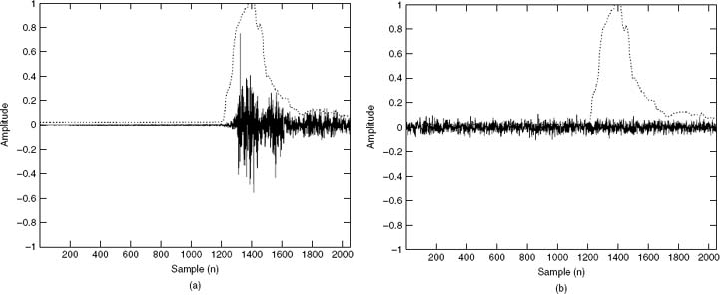
\includegraphics[scale=.6]{graph/tns.png}
            \end{figure}
			\pause
            \bigskip
            \item	\textbf{PNS} (perceptual noise substitution)
                \begin{itemize}
                    \item   transmit noise level and inter-channel correlation instead of encoding noise subbands
                \end{itemize}
		\end{itemize}
	\end{frame}
    \begin{frame}{source coding}{perceptual coding tweaks: other tools (MPEG-4 AAC, 2nd generation) 1/2}
        \begin{itemize}
			\item	\textbf{PS} (parametric stereo)
                \begin{itemize}
                    \item   extends the IS concept:
                    \item[] encode \textit{one} channel and transmit control info to generate the other channel
                \end{itemize}
		\end{itemize}
	\end{frame}
    \begin{frame}{source coding}{perceptual coding tweaks: other tools (MPEG-4 AAC, 2nd generation) 2/2}
        \begin{itemize}
            \item	\textbf{SBR} (spectral band replication)
                \begin{itemize}
                    \item encode \textit{band limited} signal and transmit control info to generate high frequency content
                \end{itemize}
		\end{itemize}
        \begin{figure}
            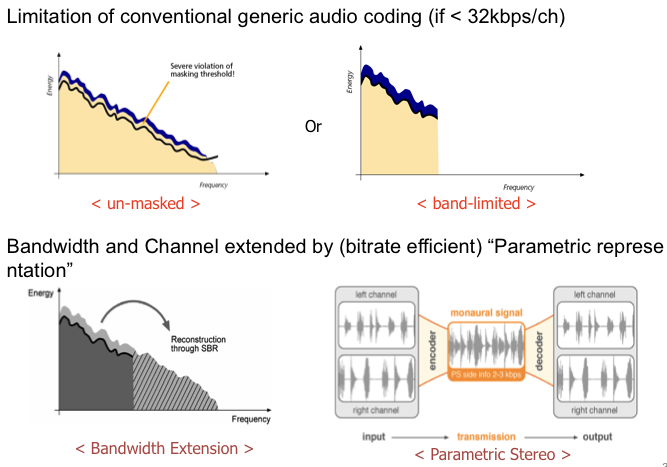
\includegraphics[scale=.5]{graph/sbr}
        \end{figure}
	\end{frame}
	
	\begin{frame}{source coding}{perceptual coding artifacts}
		\begin{itemize}
			\item	\textbf{transient smearing}\\
					transients are smoothed out
			\smallskip
            \item	\textbf{musical noise} (ringing)\\
					switch high frequency bands on and off
			\smallskip
            \item	\textbf{stereo imaging}\\
					changing localization and spatial impression
			\smallskip
            \item	\textbf{roughness}\\
					time-variant granular quantization noise
		\end{itemize}
	\end{frame}
	
	\begin{frame}{source coding}{perceptual coding audio examples (MP3)}
        \begin{columns}
            \column{.5\textwidth}
            \textbf{Harspichord}
                \begin{itemize}
                    \item   original \includeaudio{audio/mp3Original.mp3}
                    \item   \unit[256]{kbps} \includeaudio{audio/mp3_256.mp3}
                    \item   \unit[128]{kbps} \includeaudio{audio/mp3_128.mp3}
                    \item   \unit[96]{kbps} \includeaudio{audio/mp3_96.mp3}
                    \item   \unit[64]{kbps} \includeaudio{audio/mp3_64.mp3}
                    \item   \unit[32]{kbps} \includeaudio{audio/mp3_32.mp3}
                \end{itemize}
            \column{.5\textwidth}
            \textbf{Percussion}
                \begin{itemize}
                    \item   original \includeaudio{audio/Mp3_Perc_original.mp3}
                    \item   \unit[256]{kbps} \includeaudio{audio/Mp3_Perc_256.mp3}
                    \item   \unit[128]{kbps} \includeaudio{audio/Mp3_Perc_128.mp3}
                    \item   \unit[96]{kbps} \includeaudio{audio/Mp3_Perc_96.mp3}
                    \item   \unit[64]{kbps} \includeaudio{audio/Mp3_Perc_64.mp3}
                    \item   \unit[32]{kbps} \includeaudio{audio/Mp3_Perc_32.mp3}
                \end{itemize}
        \end{columns}
	\end{frame}
	
	\begin{frame}{source coding}{perceptual coding: bitrate models}
		\begin{itemize}	
			\item	\textbf{constant bit rate} (CBR):
					\begin{itemize}
						\item	bit rate constant over time
						\item	quality changes over time
					\end{itemize}
			\bigskip
            \item	\textbf{variable bit rate} (VBR):
					\begin{itemize}
						\item	bit rate changes over time
						\item	quality constant over time (depends on psychoacoustic model)
					\end{itemize}
		\end{itemize}
	\end{frame}		

	\begin{frame}{source coding}{perceptual coding algorithms}
		\begin{table}
			\begin{center}
			\begin{footnotesize}
				\begin{tabular}{lccc}
				\hline
					\textbf{Name} & \textbf{Sampling Rates}	& \textbf{Channels}	& \textbf{Bit Rates} \\
				\hline
				MPEG2 Layer 2	& 16-48k 			& 5.1 	& 8-160\\
				MPEG2 Layer 3	& 8-96k 			& 5.1 	& 8-160\\
				MPEG4 AAC	& 16-48k 			& 48.16 	& 8-320\\
				ATRAC1 	& 44.1k	& 2 	& 146\\
				ATRAC3 	& 44.1k	& 2 	& 66,33\\
				SDDS 	& 44.1k	& 7.1 	& 146\\
				AC-3 	& 32-48k 			& 5.1	& 32-640\\
				E-AC-3 	& 32-48k 			& 13.1	& 32-6144\\
				DTS (Cine) 	& 44.1k 			& 5.1/6.1	& 192\\
				DTS (Home) 	& 32-96k 			& 8	& 8-512\\
				\end{tabular}  
			\end{footnotesize}
			\end{center}
		\end{table}
	\end{frame}		

	\begin{frame}{source coding}{perceptual coding: quality evaluation 1/2}
		\begin{itemize}
			\item	quality depends on:
			\begin{itemize}
				\item	bit rate
				\item	general coding algorithm
				\item	encoder implementation!
				\item	encoder options
				\item	\color<2->{gtgold}{input signal \& its properties}
				\item	\color<2->{gtgold}{listener}
			\end{itemize}
			\pause
			$\Rightarrow$ objective, technical measures for quality evaluation fail
		\end{itemize}
	\end{frame}		

	\begin{frame}{source coding}{perceptual coding: quality evaluation 2/2}
		blind listening tests with hidden reference
		
		\only<1>{
			\begin{figure}
				\centering
					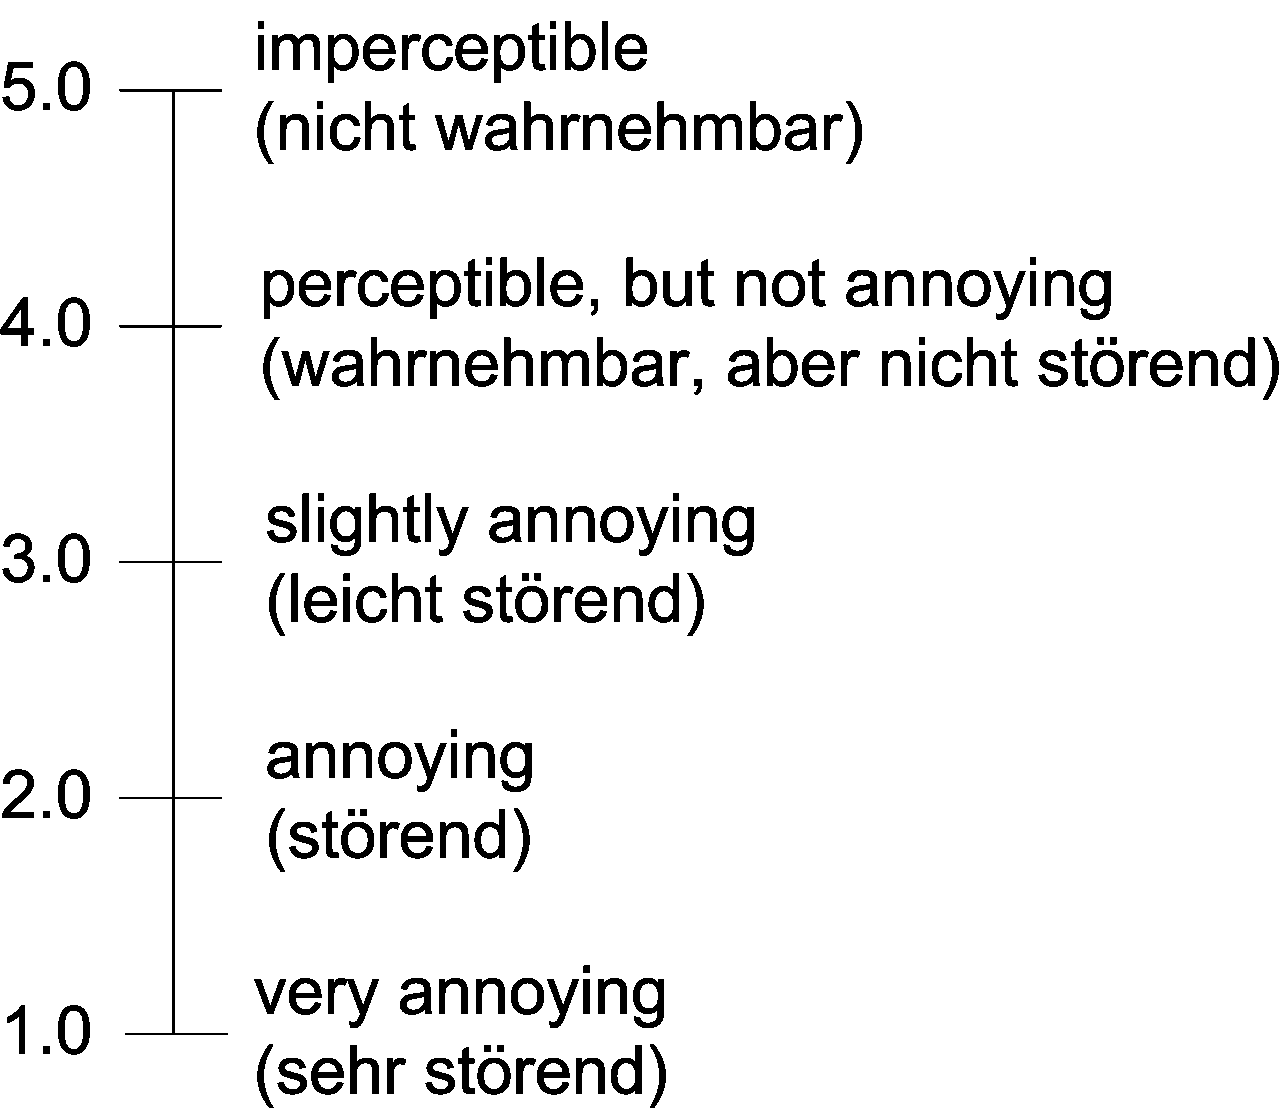
\includegraphics[scale=0.8]{graph/bewertungsscala}
			\end{figure}
			}
		\pause		
		example results
		\begin{table}
			\begin{center}
			\begin{footnotesize}
				\begin{tabular}{lccc}
				\hline
					\textbf{approach} & \textbf{SDG (app.)} \\
				\hline
				AAC/128, AC-3/192	& -0.5\\
				PAC/160	& -0.8\\
				PAC/128, AC-3/160, AAC/96, Layer 2/192	& -1.2 \ldots -1.0\\
				ITIS/192 	& -1.4\\
				Layer 3/128, Layer 2/160, PAC/96, ITIS/160 	& -1.8 \ldots -1.7\\
				AC-3/128, Layer 2/128, ITIS/128 	&  -2.2 \ldots -2.1\\
				PAC/64 	& -3.1\\
				ITIS/96 	& -3.3\\
				\end{tabular}  
			\end{footnotesize}
			\end{center}
		\end{table}
	\end{frame}		

	\begin{frame}{source coding}{perceptual coding: requirements}
        \begin{itemize}
            \item   quality (see above)
            \item	latency
                \begin{itemize}
                    \item   not important for file encoding, but for real-time transmission
                \end{itemize}
            \item	complexity
                \begin{itemize}
                    \item   encoder vs. decoder
                \end{itemize}
            \item   achievable bit rates
            \item   efficiency
                \begin{itemize}
                    \item   sound quality to bit rate
                \end{itemize}
            \item	availability and license
            \item   editability, scrolling capabilities
            \item   error resilience
		\end{itemize}
\end{frame}
